\clearpage
\section{Trh kapitálu (definice, poptávka na trhu kapitálu, nabídka na trhu kapitálu, krátkodobá
rovnováha na trhu, dlouhodobá rovnováha na trhu, úroková míra).}

\subsection{Definice}
\begin{itemize}
    \item Kapitál - statky vzniklé ve výrobě, jsou vstupy uplatňované v další výrobě
    \item Na trhu s kapitálem je ve 2 formách, fyzický a a finanční.
    \item Kapitál je vstupem i výstupem.
    \item Investice do kapitálu vyžaduje obětování přítomné spotřeby v zájmu zvýšení budoucí potřeby.
    \item K přenesení ceny kapitálového statku do ceny finálního statku slouží odpisy.
\end{itemize}

\subsection{Poptávka na trhu kapitálu}
\begin{itemize}
    \item Stejně jako u ostatních výrobních faktorů, firmy chtějí maximalizovat zisk.
    \item Maximalizují zisk, když $MRP_K=MFC_K$ (příjem z mezního produktu je stejný jako
    mezní náklad výrobního faktoru).
    \item Pokud je trh dokonale konkurenční, mezní náklady na kapitál jsou rovny úrokové sazbě $MFC=i_r$.
\end{itemize}
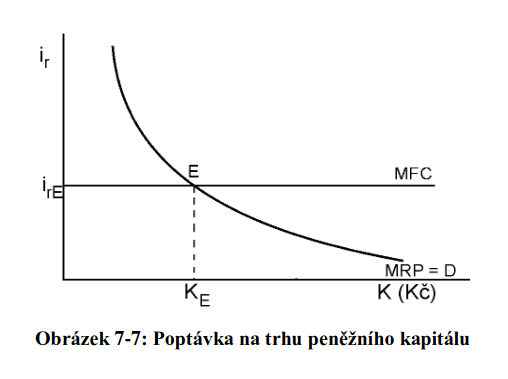
\includegraphics[width=16cm]{images/18_poptavka.png}

\subsection{Nabídka na trhu kapitálu}
\begin{itemize}
    \item Je určena výší a tvorbou úspor.
    \item Domácnosti nerady odkládají spotřebu do budoucnosti.
    \item Z krátkodobého hlediska:
    \begin{itemize}
        \item V krátkém období je daná přesná výše úspor a tím  i nabídka. Úspory jsou tedy konstantní.
    \end{itemize}
    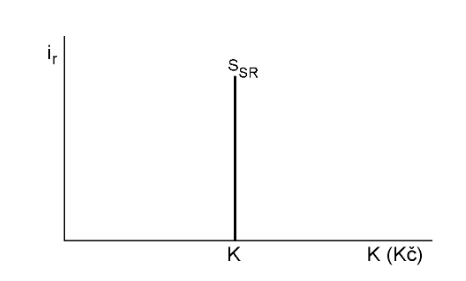
\includegraphics[]{images/18_kratkodoba_nabidka.png}
    \item Z dlouhodobého hlediska:
    \begin{itemize}
        \item Domácnosti reagují na změny úrokové sazby různou výší úspor.
    \end{itemize}
    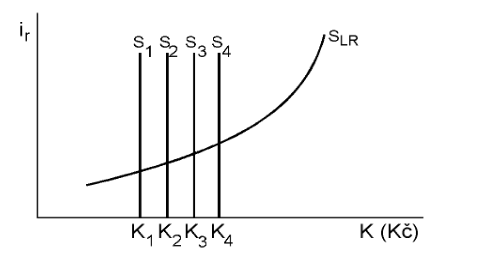
\includegraphics[]{images/18_dlouhodoba_nabidka.png}
\end{itemize}

\subsection{Krátkodobá rovnováha}
\begin{itemize}
    \item Určuje se rovnovážná úroková míra $i_r$.
    \item Průsečík nabídky a poptávky.
\end{itemize}
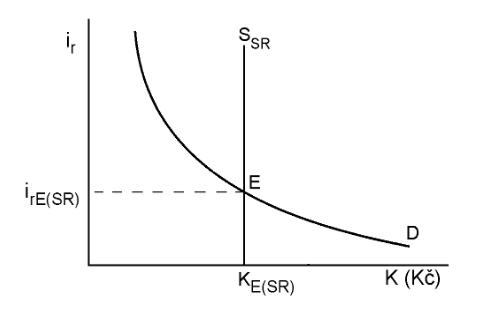
\includegraphics[width=16cm]{images/18_kratkodoba_rovnovaha.png}

\subsection{Dlouhodobá rovnováha}
\begin{itemize}
    \item Rovnovážná úroková míra vyrovná úspory a poptávku po kapitálu, podněcuje poptávku po kapitálu,
    která vyčerpá všechny úspory.
    \item Pro úrokové míry vyšší než $i_r$ platí, že domácnosti vytvářejí úspory vyšší než poptávka 
    po kapitálu.
    \item Pro úr. míry nižší platí, že poptávka po kapitálu je vyšší než vytvořené úspory.
\end{itemize}
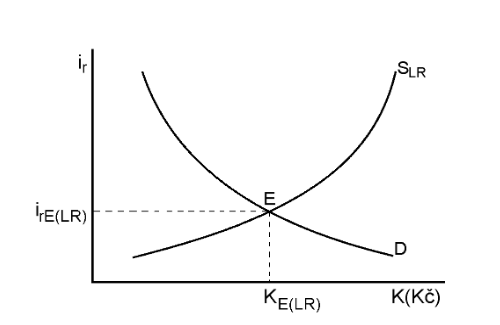
\includegraphics[width=16cm]{images/18_dlouhodoba_rovnovaha.png}

\subsection{Úroková míra}
\begin{itemize}
    \item $i=\frac{U}{K}\cdot 100 \%$, kde $i$ je roční úroková míra, $U$ je úrok, $K$ je zapůjčený kapitál.
    \item Plní funkci tržní ceny.
    \item Funkce:
    \begin{enumerate}
        \item vede domácnosti k tomu, aby obětovaly část své současné spotřeby ve prospěch
        úspor a vytvářely nabídku na trhu kapitálu
        \item podněcuje firmy k vyhledávání co nejefektivnějších investičních příležitostí
    \end{enumerate}
    \item Reálná úroková míra $i_r$: očištěná od vlivu inflace
\end{itemize}
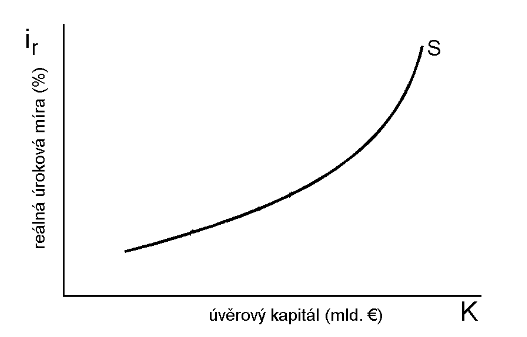
\includegraphics[width=16cm]{images/18_real_urok_m.png}